\section{Considerazioni generali}
	\subsection{Link}
	Nel sito web non si riscontra l'utilizzo di colori differenti per i link visitati 
	e per i link non ancora visitati. Tale scelta, combinata al non utilizzo 
	esplicito dei breadcrumbs, può dare vita al problema del Lost in navigation: un 
	utente, durante la navigazione, non sa più dove si trova nella gerarchia del sito 
	web, perde tempo e si arrabbia. Non colorando i collegamenti ipertestuali, 
	inoltre, si richiede all'utente uno sforzo computazionale per ricordare le pagine 
	visitate.
	Inoltre, nel web, è sempre meglio attenersi alle convenzioni e quindi colorare i
	link di colori differenti. 
	
	\subsubsection{404}
	Provando ad accedere ad una pagina inesistente oppure non più disponibile il
	sistema provvede a caricare una pagina che spiega questo errore. Tale scelta è la
	migliore possibile per questo tipo di situazioni. 
	
	\begin{figure}[H]
	\centering
	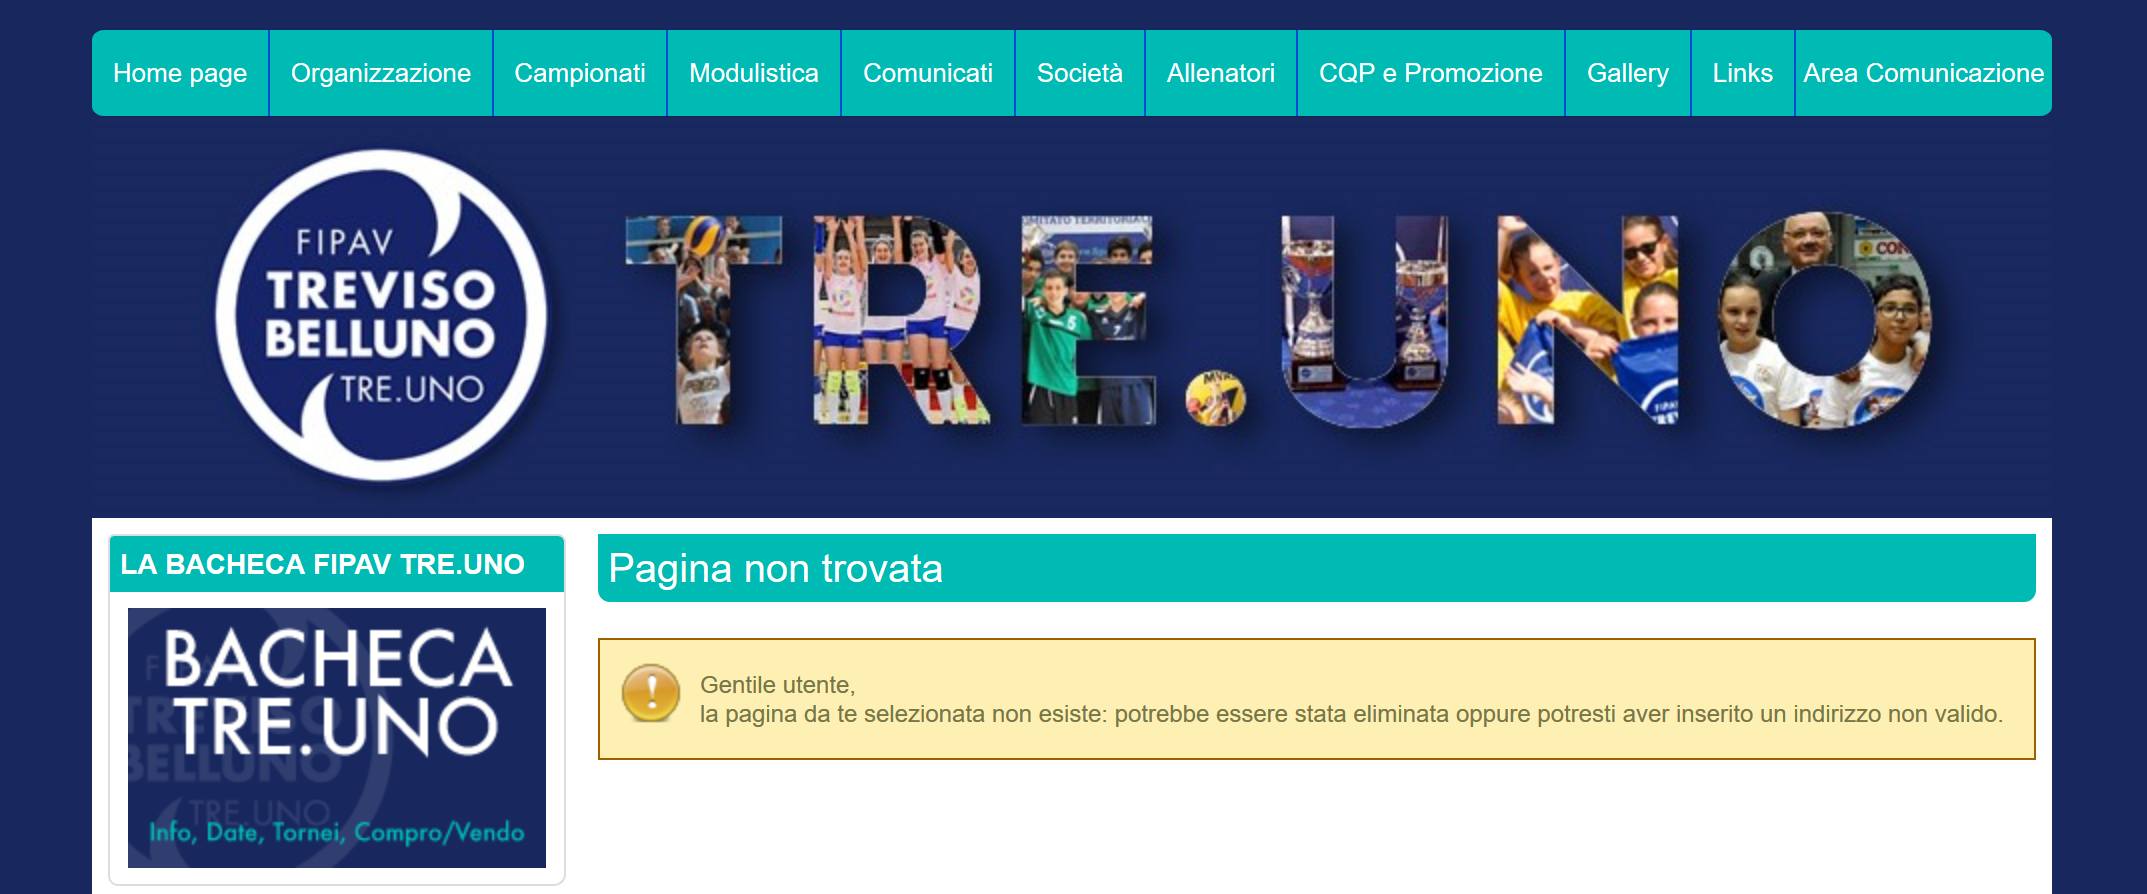
\includegraphics[scale=0.5]{Images/404.png}
	\caption{Avviso di pagina non trovata}
	\end{figure}
	
	\subsection{Apertura nuove finestre e pop-up}
	Aprendo i vari link presenti nel sito non sono state registrate aperture di nuove
	finestre e pop-up. Ciò è positivo e permette una navigazione non dispersiva.
	
	\subsection{Back button}
	Non si registrano modifiche al comportamento del tasto back del browser. Questo è
	facilitato dall'utilizzo sempre della stessa finestra di navigazione ed è
	apprezzato dagli utenti poiché abituati ad usare il back button.
	
	\subsection{Testo}
	Il testo contenuto nel sito presenta in generale una buona dimensione ed un buon 
	grado di contrasto rispetto allo sfondo: il testo normale è di colore nero su
	sfondo bianco oppure bianco su sfondo verde acqua (risulta comunque molto 
	leggibile), mentre link sono bianchi su sfondo verde acqua e quando vengono 
	selezionati il testo diventare nero e lo sfondo bianco. \\
	Il sito non offre opzioni per il resize del testo e quindi, per questo, bisogna
	affidarsi al browser. Non vengono utilizzati molti effetti nel testo. Inoltre
	viene utilizzato il grassetto per evidenziarne alcune parti. Il font utilizzato è
	il Arial, uno dei più utilizzati.
	Il testo è solitamente diviso in blocchi, ognuno dei quali contenente un
	titolo (di solito non troppo lungo). Spesso il testo presentato è veramente molto
	lungo qualora ci si trova nella sezione delle descrizioni delle società. Non è
	prevista la possibilità di cambiare lingua al sito.
	
	\subsection{Scroll}
	In generale nel sito le pagine superano di molto la grandezza consigliata
	costringendo l'utente ad effettuare molti scroll verticali. Questo problema è
	accentuato dalla scelta di presentare alcune pagine come una tabella "infinita"
	dei contenuti. Non è pervenuto invece scroll orizzontale nel caso si utilizzi 
	l'intera schermata dal desktop, ma se viene ridotta la finestra
	di navigazione, il contenuto non si adatta alle nuove misure e l'utente è 
	costretto a usare anche lo scroll orizzontale per visualizzare le informazioni 
	per intero.
	
	\begin{figure}[H]
	\centering
	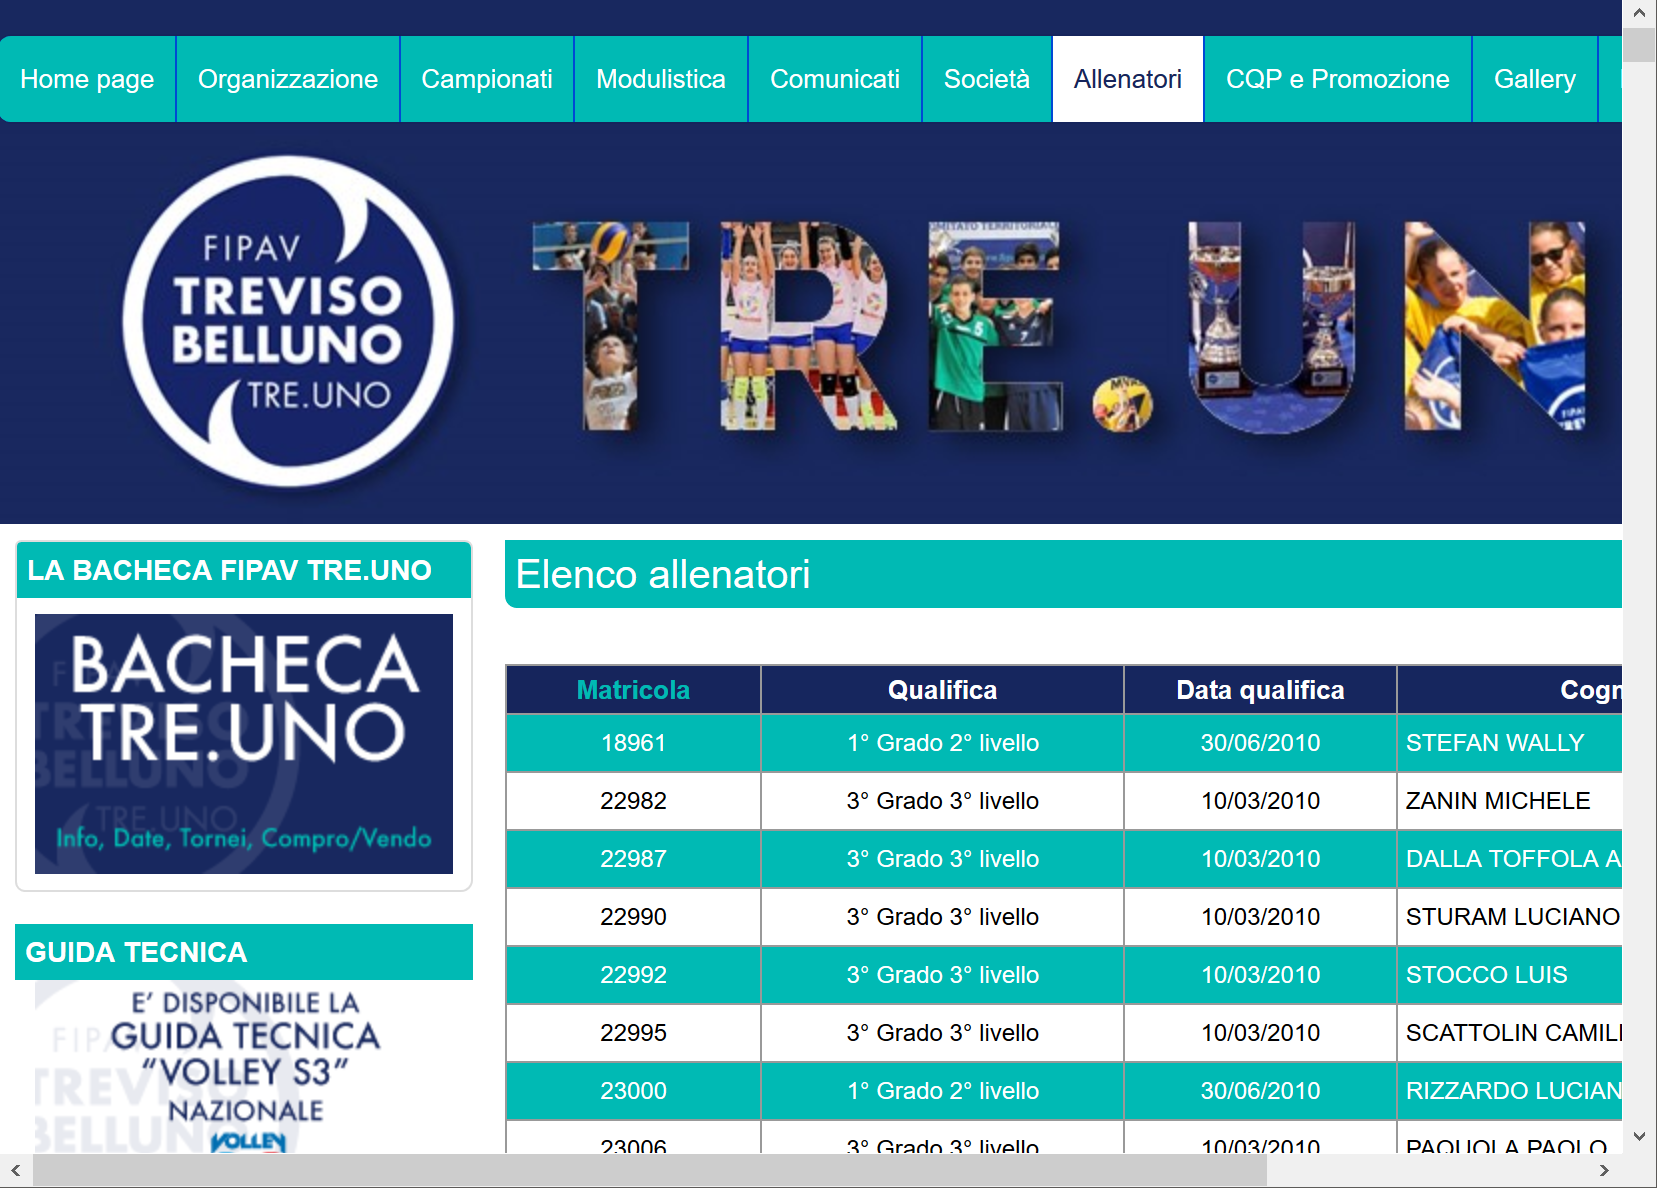
\includegraphics[scale=0.7]{Images/finestraridotta.png}
	\caption{Comparsa dello scroll orizzontale riducendo le dimensioni della 
	finestra di navigazione}
	\end{figure}
	
	
	
	